\documentclass[12pt]{article}

\usepackage{sbc-template}

\usepackage{graphicx,url}

\usepackage[brazil]{babel}
%\usepackage[latin1]{inputenc}
\usepackage[utf8]{inputenc}
% UTF-8 encoding is recommended by ShareLaTex

\usepackage{hyperref}

\usepackage{pdftexcmds}
\usepackage{minted}

%\setminted{frame=lines}

\sloppy

\title{Bancos de Dados Geográficos}

\author{Fuad Saud\inst{1}, Luiz Felipe Cunha\inst{1}, Marcel Mossmann \inst{1}, Ramon Saraiva\inst{1}}

\address{Universidade do Vale do Rio dos Sinos
  \email{\{fuadfsaud,felipe.silvacunha,marcelmossmann,ramonsaraiva\}@gmail.com}
}

\begin{document}

\maketitle

\begin{abstract}
  This paper gives an overview of the state of the art GIS-aware database
  management systems and introduces the PostGIS extension to the popular
  open source RDBMS PostgreSQL by means of examples.
\end{abstract}

\begin{resumo}
  Este artigo apresenta um apanhado do estado da arte com relação a sistemas de
  gerenciamento de bancos de dados com suporte a processamento geográfico e
  introduz o PostGIS, uma extensão do popular SGBDR PostgreSQL.
\end{resumo}


\section{Bancos de Dados Geográficos}

Por muito tempo, desde os primeiros dias dos sistemas de informação
geográficas, dados espaciais foram e ainda são armazenados em
\textit{shapefiles} - arquivos onde os dados são estruturados de forma plana
(não indexada) e que não oferecem nenhum tipo de acesso padronizado.

Utilizar um banco de dados relacional para o armazenamento e mediação de acesso
a dados geográficos oferece um leque de vantagens sobre estratégias de
armazenamento. Entre elas estão o uso do SQL como interface padrão para
interação com o banco de dados, o que permite tanto descrever computações e
relacionamentos complicados entre os dados de maneira simplificada como
combinar essas computações com outras computações relacionais triviais, levando
em conta todas as ferramentas existentes para trabalhar com bancos de dados
relacionais; acesso concorrente controlado de forma a evitar possíveis
corrupções na estrutura de armazenamento.

\section{PostGIS} \label{sec:firstpage}

Neste artigo abordaremos o \href{http://postgis.net}{PostGIS}, uma
extensão que adiciona a capacidade de trabalhar com dados geográficos ao SGBDR
PostgreSQL. A primeira versão do projeto foi publicada em 2001 pela
\href{http://refractions.net}{Refractions Research} projeto de código aberto
foi publicada em 2001 sob a GNU General Public License, permitindo a aberta
distribuição do código-fonte e uso do programa.

A partir desta versão inicial, algumas funções foram padronizadas pelo Open
Geospatial Consortium, formando a especificação SFSQL ("Simple Features for
SQL"), que posteriormente passou a ser desenvolvida de maneira independente ao
PostGIS.

\subsection{Configuração}

A instalação da extensão é deveras fácil e pode ser feita em diferentes
plataformas de várias maneiras, como descrito na
\href{http://postgis.net/install}{Apágina de instalação do site oficial}.

Uma vez instalada, a extensão pode ser habilitada em uma base de dados por meio
do seguinte comando:

\begin{minted}{sql}
  CREATE EXTENSION postgis;
\end{minted}

Dados geográficos podem ser inseridos de várias modos. Uma maneira conveniente
é importar um shapefile inteiro para a base de dados, tarefa que pode ser
realizada com a ajuda da ferramenta \texttt{shp2pgsql}. Ela transforma um
shapefile em um script SQL que pode ser rodado diretamente na base de dados com
o PostGIS habilitado da seguinte forma:

\begin{minted}{shell}
  shp2pgsql /path/to/shapefile.shp > output.sql
  pgsql postgis_enabled_database < output.sql
\end{minted}

Seguem algums exemplos de funções geográficas que são implementadas pelo
PostGIS:

\begin{minted}{sql}
boolean ST_Crosses(geometry g1, geometry g2)
-- Retorna true caso as geometrias tenham alguns pontos internos
-- em comum, mas não todos.

geometry ST_Difference(geometry g1, geometry g2)
-- Retorna a diferença entre a geometria 1g em relação a g2,
-- isto é, os pontos de g1 que não fazem partde de g2.

float ST_Distance(geometry g1, geometry g2)
-- Retorna a distância mínima, em um plano 2D, entre as geometrias.

boolean ST_Contains(geometry g1, geometry g2)
-- Retorna true se, e somente se, g2 não possuir nenhum
-- ponto que esteja no exterior de g1 e pelo menos um
-- ponto no interior de g1.

boolean ST_Covers(geometry g1, geometry g2)
-- Retorna true se nenhum ponto de g2 estiver fora de g1.

boolean ST_Equals(geometry g1, geometry g2)
-- Retorna true caso ambos parâmetros representem a mesma
-- geometria, ignorando a direção.

geometry ST_Intersection(geometry g1, geometry g2)
-- Retorna uma geometria contendo os pontos em comum entre g1 e g2.

boolean ST_Intersects(geometry g1, geometry g2)
-- Retorna true caso g1 e g2 compartilhem qualquer porção de espaço.

boolean ST_IsValid(geometry g)
-- Retorna true caso a geometria seja bem formada. Caso seja
-- inválida, o PostgreSQL notice irá disponibilizar detalhes da razão.

float ST_Length(geometry a_2dlinestring)
-- Retorna  o comprimento 2D da geometria, caso seja uma LineString ou
-- MultiLineString.

boolean ST_Overlaps(geometry g1, geometry g2)
-- Retorna true caso as geometrias dividam espaço, sejam de mesma
-- dimensão, porém não sejam completamente contidas pela outra.

float ST_Perimeter(geometry g1)
-- Retorna a medida do comprimento dos limites de um ST_Surface
-- ou ST_MultiSurface.
\end{minted}

\section{Indexação}
Um banco de dados geospacial somente é possível se existir algum tipo de indexação
espacial, pois sem ela não há forma de o banco realizar consultas em tempo real.
Sem este tipo de indexação um join entre duas tabelas com 10.000 registros cada,
executaria um total de 100.000.000 comparações, no entanto com indexação espacial
nas duas tabelas o número de comparações pode cair para aproximadamente 20.000.

O postgis possui, além da indexação tradicional do PostgreSQL, um sistema de
indexação espacial chamado GiST (Generalized Search Tree) sobre uma
árvore R-Tree, que pode ser criado da seguinte forma:
\begin{minted}{sql}
  CREATE INDEX [indexname]
    ON [tablename]
    USING GIST ( [geometryfield] );
\end{minted}

Por padrão será criado um índice de 2 dimensões, para criar um índice de N dimensões:
\begin{minted}{sql}
  CREATE INDEX [indexname]
    ON [tablename]
    USING GIST ([geometryfield] gist_geometry_ops_nd);
\end{minted}

\subsection{Funcionamento}
O GiST funciona com um sistema de \textit{bounding boxes} (Figura~\ref{fig:indexes_bbox}),
ou seja, para cada polígono armazenado é criada o menor retângulo possível que o
compreenda, estes novos polígonos menos complexos são armazenados na estrutura hierarquica
de indexação.

\begin{figure}[ht]
  \centering
  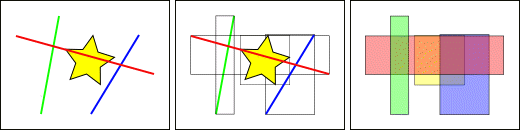
\includegraphics[width=1\textwidth]{indexes_bbox.png}
  \caption{Bounding boxes}
  \label{fig:indexes_bbox}
\end{figure}

Então para realizar uma busca de polígonos que se intersecionam, primeiro é realizada a
verificação de quais retângulos se intersecionam, e somente é realizado o cálculo de
intersecção dos polígonos complexos nas intersecções dos retêngulos, desta forma temos uma
menor complexidade para calcular as intersecções entres os polígonos.

\subsection{Esturura hierárquica - GiST + R-Tree}
O postgis armazena os retângulos em uma árvore (Figura~\ref{fig:indexes_rtree}) de N
níveis de acordo com a densidade de polígonos, afim de reduzir a complexidade de busca.
Desta form ele cria novos retângulos lógicos, de forma automática, que compreendem
retângulos referentes a polígonos complexos, de tal forma a criar uma estrutura hierárquica
de retângulos, onde os retângulos referentes a polígonos complexos ficam armazenados nas
folhas e os retângulos lógicos no restante da árvore. Desta forma o caminhamento na árvore
em busca de polígonos complexos é mínimo.

\begin{figure}[ht]
  \centering
  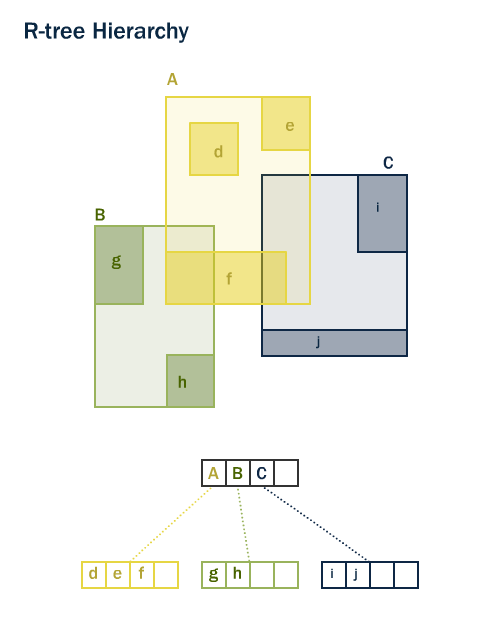
\includegraphics[width=.5\textwidth]{indexes_rtree.png}
  \caption{Indexação de retângulos R-Tree}
  \label{fig:indexes_rtree}
\end{figure}
\section{Implementação}

Para exemplificar os conceitos descritos foi realizada a implmentação de uma
aplicação Web que pode ser acessada na seguinte URL:
\url{http://ramonsaraiva.xyz}. O código da aplicação está disponível no
seguinte endereço: \url{https://github.com/ramonsaraiva/unigis}.

A implementação é escrita em Python e JavaScript e utiliza o ORM GeoAlchemy.

\section{Conclusão}

O PostGIS é uma solução robusta e moderna para armazenamento, busca e indexação
de dados geoespaciais, que por estar aliado a confiabilidade, extensibilidade e
ao ecossistema do PostgreSQL se torna um produto extremamente popular e
acessível para uso em aplicações em geral.

\bibliographystyle{sbc}
\bibliography{geodb}
\nocite{*}

\end{document}
